\chapter{Implementationsdetails}
\label{chap:implementierung}
In diesem Kapitel werden das die Funktionalitäten der Pipeline zusammengetragen. Um die Anforderungen genauer zu beschreiben, wird ein Use-Case-Diagramm und ein Klassendiagramm dargestellt und beschrieben. Zudem werden konkrete funktionale und nichtfunktionale Anforderungen des Systems erfasst. Abschließend werden verwendete Technologien und Implementationsaspekte genauer beschrieben.
\section{Beschreibung des entwickelten Systems}
\label{sec:beschreibungsystem}
Es wird eine Lösung gesucht, die eine effiziente Verarbeitung von \emph{Bedarfsmeldungen} durchführen kann. Welche Aspekte in einer Bedarfsmeldung relevant sind, wurde bereits im Kapitel \ref{chap:erwartungshaltung} näher erläutert. Auf Basis welcher Methodiken und Ansätze die relevanten Informationen extrahiert werden können, wurde in Kapitel \ref{sec:literaturueberblick} dargestellt. Nun gilt es eine Lösung zu entwickeln, die diese Ansätze in einem System implementiert und Möglichkeiten zur Evaluation bietet. Die Idee ist es, eine Pipeline zu entwickeln, die Möglichkeiten zum laden von \emph{Bedarfsmeldungen} hat. Damit alle Ansätze und Methoden zur Extraktion von Informationen gut funktionieren und vergleichbar bleiben, wird eine Übersetzungsfunktion der \emph{Bedarfsmeldungen} benötigt. Auch wenn die \emph{Bedarfsmeldungen} in den meisten Fällen auf Deutsch sind, hilf es diese zu übersetzen, damit keine Unterschiede in der Ergebnisqualität resultiert, da einige Methoden und Ansätze auf Basis von Englischen Trainingssätzen trainiert wurden. Schließlich müssen alle aus Kapitel \ref{sec:literaturueberblick} untersuchten Ansätze implementiert und nutzbar ein. Sie sollen die Möglichkeit haben \emph{Bedarfsmeldungen} als Input zu erhalten und eine Ausgabe zurückzugeben. Zur besseren Evaluationsmöglichkeit soll das System modular sein, damit Methoden und Ansätze nach belieben durchgetauscht werden können. Zur Überprüfung der Laufzeit soll eine Zeitmessung verfügbar sein, die die Zeit zwischen dem Start und der Beendigung des Systems zurückgibt.\\

\todo{erzählen was die Pipeline leisten soll, im Falle vom Hybrid wird wahrscheinlich noch data-fusion gebraucht, vektorisierung eventuell auch noch für cosine similarity}
\newpage
\section{Use-Case}
\label{sec:usecase}
In diesem Kapitel werden die Interaktionen zwischen Benutzer und System beschrieben. Dazu wird ein Use-Case-Diagramm angefertigt, das eine grafische Übersicht über alle Anwendungsfälle bietet.
\begin{figure}[H]
	\centering  
	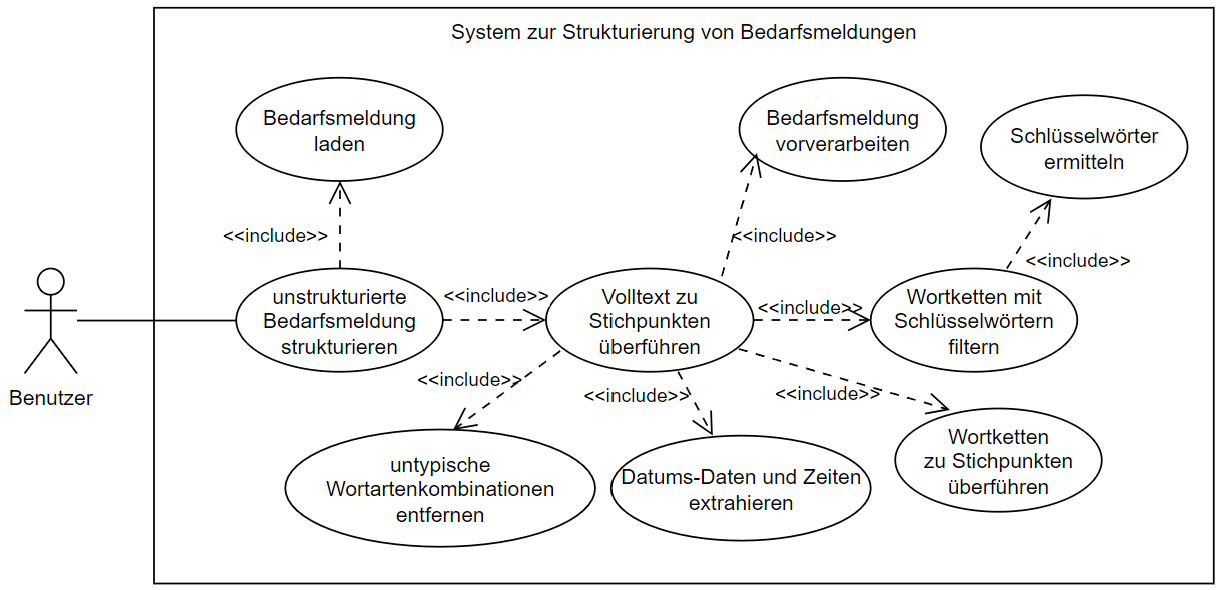
\includegraphics[width=\linewidth]{Abbildungen/use-case.png}
	\caption{Use-Case Diagramm der Pipeline.}
	\label{fig:usecasediagrammwirklich}
\end{figure}\mbox{} \\
\todo{use case beschreiben}
%Es existieren zwei Akteure mit differenzierten Rechten. Beide authentifizieren sich zu Beginn auf der Anmeldeseite. Einer der beiden Akteure ist der Benutzer, der die Option hat, eine Bedarfsmeldung aus JIRA auszuwählen oder in einem Freitext eine eigene Anforderung zu hinterlegen. Anschließend kann die Bedarfsmeldung entweder zur Schlüsselwörterüberprüfung oder direkt an die KI-Schnittstelle gesendet werden. Der zweite Akteur ist der Admin. Dieser hat Zugriff auf alle Funktionalitäten, die der Benutzer verwenden darf. Darüber hinaus stehen diesem auf dem \emph{Dashboard} visualisierende und vergleichende Methoden des KI-Ansatzes zur Verfügung.
\section{Anforderungen}
Im Folgenden werden die funktionalen sowie nichtfunktionalen Anforderungen des Systems beschrieben. Diese Informationen wurden aus der Beschreibung des Systems aus Kapitel \ref{sec:beschreibungsystem} und dem Use-Case aus Kapitel \ref{sec:usecase} hergeleitet und bilden den Rahmen des Systems.
\subsection{Funktionale Anforderungen}
Die funktionalen Anforderungen beschreiben konkrete Funktionalitäten des Systems. Dazu werden zusammengehörende Anforderungen nummeriert und im Falle der Systemanforderungen in detaillierte Unterpunkte aufgelistet und beschrieben.
\paragraph{Benutzeranforderungen}
\begin{enumerate}
	\item Dem Benutzer soll es möglich sein, Extraktionsmethoden austauschen zu können.
	\item Dem Benutzer soll es möglich sein, die Laufzeit des Systems zu sehen.
\end{enumerate}
\todo{vielleicht dann auch die evaluationsschritte einbauen}
\paragraph{Systemanforderungen}
\begin{enumerate}[label=1.\arabic*]
	\item Die \emph{Bedarfsmeldungen} sollen geladen werden können.
	\item Beim laden können eine oder mehrere \emph{Bedarfsmeldungen} geladen werden.
	\item Das System soll die Datenformate \emph{.txt} und \emph{.json} unterstützen.
\end{enumerate}
\begin{enumerate}[label=2.\arabic*]
	\item Die Bedarfsmeldungen sollen ins Englische übersetzt werden können.
\end{enumerate}
\begin{enumerate}[label=3.\arabic*]
	\item Das System soll Methoden des Preprocessing zur Bereinigung eines Volltextes implementiert haben.
	\item Das Preprocessing soll ein Volltext als Eingabe erhalten.
	\item Das Preprocessing soll den Volltext als Ausgabe zurückgeben.
\end{enumerate}
\begin{enumerate}[label=4.\arabic*]
	\item Das System soll die Methode \emph{TF-IDF} als Modul implementiert haben.
	\item Das Modul soll die Möglichkeit haben ein Volltextes als Eingabe für die implementierte Methode mitzugeben.
\end{enumerate}
\begin{enumerate}[label=5.\arabic*]
	\item Das System soll die Methode \emph{TextRank} als Modul implementiert haben.
	\item Das Modul soll die Möglichkeit haben ein Volltextes als Eingabe für die implementierte Methode mitzugeben.
\end{enumerate}
\begin{enumerate}[label=6.\arabic*]
	\item Das System soll die Methode \emph{N-Gram} als Modul implementiert haben.
	\item Das Modul soll die Möglichkeit haben ein Volltextes als Eingabe für die implementierte Methode mitzugeben.
\end{enumerate}
\begin{enumerate}[label=7.\arabic*]
	\item Das System soll die Methode \emph{POS-Tagging} als Modul implementiert haben.
	\item Das Modul soll die Möglichkeit haben ein Volltextes als Eingabe für die implementierte Methode mitzugeben.
\end{enumerate}
\begin{enumerate}[label=8.\arabic*]
	\item Das System soll die Methode \emph{NER} als Modul implementiert haben.
	\item Das Modul soll die Möglichkeit haben ein Volltextes als Eingabe für die implementierte Methode mitzugeben.
\end{enumerate}
\begin{enumerate}[label=8.\arabic*]
	\item Das System soll die Möglichkeit haben die Laufzeit des Systems zu messen.
	\item Der Startzeitpunkt wird beim Systemstart festgehalten.
	\item Der Endzeitpunkt wird beim Systemstop festgehalten.
	\item Die Differenz aus dem Start- und Stop- Zeitpunkt wird ermittelt.
\end{enumerate}
\subsection{Nichtfunktionale Anforderungen}
Hierbei handelt es sich um qualitätsbezogene Anforderungen. Diese umfassen nicht konkrete Funktionen des Systems, sondern stellen Rahmenbedingungen des Systems im Ganzen zusammen.
\begin{enumerate}
	\item Das System soll modular aufgebaut sein, um die Extraktionsmethoden austauschen zu können.
	\item Das System soll in der Lage sein, mehrere \emph{Bedarfsmeldungen} laden zu können.
\end{enumerate}
\newpage
\section{Systemablauf}
\todo{Flussdiagramm beschreiben und in der Einleitung nicht vergessen im Ablauf anzupassen dass das kein Klassendiagramm mehr ist}
\begin{figure}[H]
	\centering  
	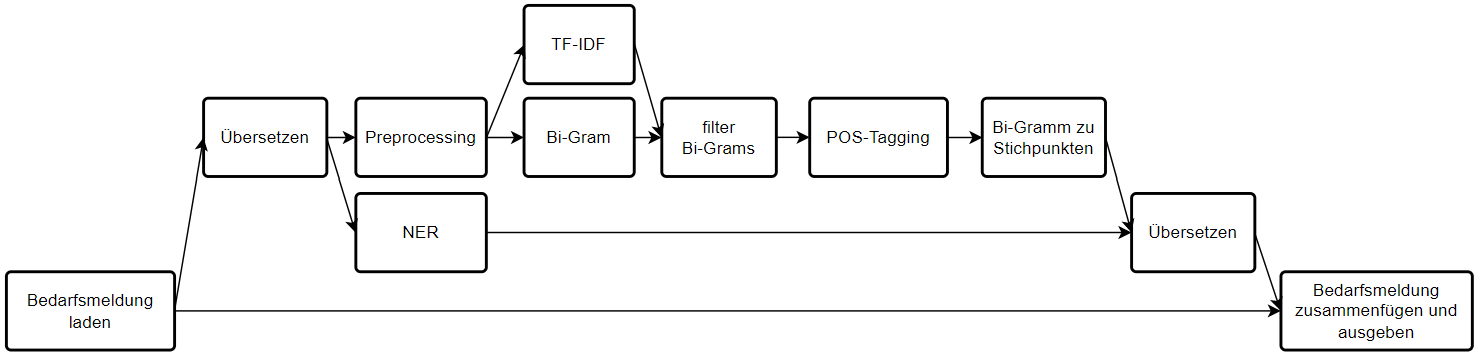
\includegraphics[width=\linewidth]{Abbildungen/flowchart.png}
	\caption{Flussdiagramm der Pipeline.}
	\label{fig:flowchart}
\end{figure}\mbox{} \\
\newpage
\section{Details zur Implementierung der Pipeline}
Dieses Kapitel beschreibt den technischen Entwicklungsprozess zur Umsetzung der Anforderungen des Systems. Die Implementierung fokussiert sich auf die Umsetzungen von Technologien und Funktionsweisen verschiedener Anforderungen. Zudem wird die Struktur des Projektes aufgezeigt.
\subsection{Umsetzung}
in python - warum, modular
\subsection{Projektstruktur}
Das Projekt wird in einem git Repository gespeichert und versioniert. Die Projektstruktur ist ohne zusätzliche Konfigurationsdateien wie folgt aufgebaut:
\dirtree{%
	.1 .git/.
	.2 modules/.
	.3 nGram.py.
	.3 posTagging.py.
	.3 preprocessing.
	.3 ner.py.
	.3 textRankingArgorithm.py.
	.3 tfIdf.py.
	.2 requirements/.
	.3 syntheticData.txt.
	.3 syntheticData.json.
	.3 ....
	.2 app.py.
	.2 ....
}
\url{client/}-Verzeichnis

\subsection{Modulimplemetierungen}
Das Ziel der Arbeit besteht nicht in der Erweiterung der Verfahren, sondern in der Evaluierung ihrer Eignung zur Extraktion relevanter Informationen aus Bedarfsmeldungen. Die Prüfung erfolgt ohne die Notwendigkeit der Entwicklung und Testung neuer Systeme. Es existieren bereits Bibliotheken mit Implementierungen.
\paragraph{Dateiformat}

\paragraph{Übersetzung}

\paragraph{Preprocessing}

\paragraph{TF-IDF}

\paragraph{TextRank}

\paragraph{N-Gramm}

\paragraph{POS-Tagging}

\paragraph{NER}

\paragraph{data-fusion}